\RequirePackage[l2tabu, orthodox]{nag}
\documentclass[french]{beamer}
\usetheme{Madrid}
%\usetheme{metropolis}
\usefonttheme{professionalfonts}

\usepackage{standalone, import} % \subimport*{relative/}{file} or \subincludefrom*{relative/}{file}
\usepackage{xspace, calc, tikz}
\usepackage[autolanguage]{numprint}
%\usepackage{siunitx} % See https://github.com/wspr/unicode-math/issues/318
\usepackage{babel}
\usepackage{mathtools, amssymb}
\usepackage[normalem]{ulem} % strikethrough (\sout)
\usepackage[perpage]{footmisc}
\usepackage[all]{nowidow}
\usepackage[justification=centering]{caption}
\usepackage{graphicx, grffile, subcaption} % Images in \adjustimage{k=v}{file} ; subfloat in env 'subfigure'
\usepackage{float, placeins} % Floats stay before or after \FloatBarrier, prefer to [H]
\usepackage{ltablex, booktabs, tabulary} %ltablex: 'tabularx' as longtables ; autoresize columns in tabulary
%\usepackage[modulo]{lineno} % N° de ligne dans \begin{linenumbers}
%\usepackage{lipsum} % Lorem ipsum dans \lipsum
%\usepackage{pdflscape}
%\usepackage{verse, attrib} % Format poems
\usepackage{multicol} %\begin{columns}{<nbColonnes>}[<Texte avt colonne>]{<txt> \columnbreak <txt>}
%\usepackage[backend=biber, doi=false, url=false]{biblatex}
\usepackage{fvextra, verbatim} % {Verbatim}
%\usepackage{minted} % in {minted}[opt]{lang}
%\fvset{linenos}
\usepackage{suffix}
\usepackage{relsize}

\usepackage{fontspec, realscripts, metalogo}
%\setmainfont[SmallCapsFont={Latin Modern Roman Caps},Ligatures=TeX]{Latin Modern Roman}
\setmainfont{STIX Two Text}
\setsansfont{Fira Sans}
\usepackage[math-style=french]{unicode-math}
%\setmathfont{Latin Modern Math}
\setmathfont{STIX Two Math}

\usetikzlibrary{matrix}
\usepackage[strict]{csquotes}
\usepackage{microtype}
\usepackage{trace}

%\addbibresource{base.bib}
\title[Comportement d'un mélange phénol-eau]{Comportement d'un mélange phénol-eau :\\une approche statistique}
\author{Valentin \texorpdfstring{\bsc{Ogier}}{Ogier}}
\date{2018}

\newcommand{\p}[1]{\mintinline{python3}{#1}}

\DeclareMathOperator{\bsum}{\mathlarger{\sum}}
\DeclareMathOperator{\bbsum}{\mathlarger{\mathlarger{\sum}}}

\DeclareMathOperator{\bord}{bord}

%%% Autotitle slides.
\addtobeamertemplate{frametitle}{
	\let\insertframetitle\insertsectionhead}{}
\addtobeamertemplate{frametitle}{
	\let\insertframesubtitle\insertsubsectionhead}{}

\makeatletter
\CheckCommand*\beamer@checkframetitle{\@ifnextchar\bgroup\beamer@inlineframetitle{}}
\renewcommand*\beamer@checkframetitle{\global\let\beamer@frametitle\relax\@ifnextchar\bgroup\beamer@inlineframetitle{}}
\makeatother
%%%


\begin{document}
\frame{\titlepage}
\frame{\tableofcontents}
	
%%%
\section{Mise en situation}
\subsection{Introduction}
%%%

\begin{frame}
    \begin{figure}
        \centering
        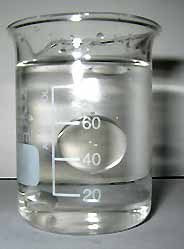
\includegraphics[height=0.65\textheight]{assets/miscibilite-bulle}
        \caption{Bulle d'huile dans un mélange eau-alcool}
        \label{fig:miscibilite-bulle}
    \end{figure}
\end{frame}

\subsection{Le modèle d'\bsc{Ising}}

\begin{frame}
\begin{figure}
	\centering
	\begin{tikzpicture}[ampersand replacement=\&]
	\fill[blue!40!white] (-3,-3) rectangle (3,-2);
	\fill[blue!40!white] (-3,-3) rectangle (-2,3);
	\fill[blue!40!white] (2,-2) rectangle (3,3);
	\fill[blue!40!white] (-2,2) rectangle (3,3);
	\draw[step=1cm,color=gray] (-3,-3) grid (3,3);
	
	\matrix[matrix of nodes,nodes={inner sep=0pt,text width=1cm,align=center,minimum height=1cm}]{
		$+1$ \& $+1$ \& $+1$ \& $+1$ \& $+1$ \& $+1$ \\
		$+1$ \& $+1$ \& $-1$ \& $-1$ \& $+1$ \& $+1$ \\
		$+1$ \& $-1$ \& $+1$ \& $+1$ \& $-1$ \& $+1$ \\
		$+1$ \& $-1$ \& $-1$ \& $+1$ \& $-1$ \& $+1$ \\
		$+1$ \& $-1$ \& $-1$ \& $+1$ \& $+1$ \& $+1$ \\
		$+1$ \& $+1$ \& $+1$ \& $+1$ \& $+1$ \& $+1$ \\
	};
	\end{tikzpicture}
	\caption{Une configuration $\sigma$ sur un treillis $6\times6$ avec condition de bords $+$}
\end{figure}
\end{frame}


\begin{frame}
    \begin{itemize}
        \item un graphe \(G\) (\(\subseteq \mathbb{Z}^d\))
        \item une configuration \(\sigma : V_G \to \left\{-1, +1\right\} \)
        \item fonction donnant l'énergie totale d'une configuration (Hamiltonien) :
        \[
        \forall \sigma \in \left\{-1, +1\right\} \qquad H(\sigma) = - J \sum_\text{$i$, $j$ voisins} \sigma(i)\sigma(j)
                 - J \sum_{i \in \bord(G)} \sigma(i)
        \]
        où \(J > 0\) est une constante correspondant à l'énergie d'interaction entre deux molécules et
        \[
        \bord(G) = \left\{x \in V_G \mid \exists y \in \mathbb{Z}^d\setminus V_G, \text{$x$ et $y$ voisins} \right\}
        \]
    \end{itemize}
\end{frame}




\begin{frame}
\begin{figure}
    \centering
    \begin{tikzpicture}[ampersand replacement=\&]
    \fill[blue!40!white] (-3,-3) rectangle (3,-2);
    \fill[blue!40!white] (-3,-3) rectangle (-2,3);
    \fill[blue!40!white] (2,-2) rectangle (3,3);
    \fill[blue!40!white] (-2,2) rectangle (3,3);
    \draw[step=1cm,color=gray] (-3,-3) grid (3,3);

    \matrix[matrix of nodes,nodes={inner sep=0pt,text width=1cm,align=center,minimum height=1cm}]{
        $+1$ \& $+1$ \& $+1$ \& $+1$ \& $+1$ \& $+1$ \\
        $+1$ \& $+1$ \& $-1$ \& $-1$ \& $+1$ \& $+1$ \\
        $+1$ \& $-1$ \& $+1$ \& $+1$ \& $-1$ \& $+1$ \\
        $+1$ \& $-1$ \& $-1$ \& $+1$ \& $-1$ \& $+1$ \\
        $+1$ \& $-1$ \& $-1$ \& $+1$ \& $+1$ \& $+1$ \\
        $+1$ \& $+1$ \& $+1$ \& $+1$ \& $+1$ \& $+1$ \\
    };
    \end{tikzpicture}
    \caption{Une configuration $\sigma$ sur un treillis $6\times6$ avec condition de bords $+$}
\end{figure}
\end{frame}

\begin{frame}
    \begin{definition}[Mesure de \bsc{Gibbs}]
    Dans l'ensemble canonique à la température inverse $\beta = \frac{1}{k_BT}$, la probabilité d'être dans la configuration \(\sigma\)  est donnée par
        \[\mu_\beta(\sigma) = \frac{e^ { - \beta H(\sigma)}}{Z_\beta} \]
        où $Z$ est la fonction de partition définie par \[Z_\beta = \sum_{\sigma \in \left\{-1, +1\right\}^{V_G}} e^{-\beta H(\sigma)}\]
    \end{definition}
\end{frame}

%%%
\section{Transition de phase}
\subsection{Définition}
%%%

\begin{frame}
    On cherche la température inverse critique $\beta_C$ telle que
    \begin{itemize}
        \item si $\beta < \beta_C$, le mélange est homogène
        \item si $\beta > \beta_C$, deux phases distinctes coexistent
    \end{itemize}
    $\beta_C$ est la température inverse de la transition de phase.
    
    Comment repérer la transition de phase ?
\end{frame}

\begin{frame}
\begin{definition}[Mesure de probabilité]
    Soit $f : \left\{-1, +1\right\}^{V_G} \to \mathbb{R}$ une grandeur physique. La mesure de probabilité de $f$ à la température inverse $\beta$ est
    \[ \left\langle f \right\rangle_\beta = \sum_{\sigma \in \left\{-1, +1\right\}^{V_G}} f(\sigma)\mu_\beta(\sigma)\]
\end{definition}
La transition de phase est repérée par une discontinuité (ou forte variation) d'une mesure de probabilité.

\begin{example}
    La magnétisation spontanée $m_\beta = \left\langle \sigma(0) \right\rangle_\beta$. (pour $\beta < \beta_C$, $m_\beta = 0$ et pour $\beta > \beta_C$, $m_\beta > 0$ avec conditions aux bords $+$)
\end{example}
\end{frame}

%
\subsection{En une dimension}
%

\begin{frame}
\begin{figure}
    \centering
    \begin{tikzpicture}
\fill[blue!40!white] (-4,0) rectangle (-3,1);
\fill[blue!40!white] (3,0) rectangle (4,1);
\draw[step=1cm,color=gray] (-4,0) grid (4,1);
\node at (-3.5,+0.5) {$+1$};
\node at (-2.5,+0.5) {$-1$};
\node at (-1.5,+0.5) {$+1$};
\node at (-0.5,+0.5) {$-1$};
\node at (0.5,+0.5) {$-1$};
\node at (1.5,+0.5) {$+1$};
\node at (2.5,+0.5) {$-1$};
\node at (3.5,+0.5) {$+1$};
    \end{tikzpicture}
    \caption{Une configuration $\sigma$ avec condition de bords $+$, $N = 6$}
\end{figure}

En une dimension, sur un graphe de longueur $N$, le Hamiltonien devient
\begin{align*}
&H(\sigma) = -J \sum_{i = 1}^{N - 1} \sigma(i) \sigma(i + 1) - J \sigma(1) -J\sigma(N) \\
 \forall \sigma \in &\left\{-1, +1\right\}^N,\\
&e^{-\beta H(\sigma)} = (e^{K\sigma(1)})(e^{K\sigma(1)\sigma(2)}) (e^{K\sigma(2)\sigma(3)}) \dots (e^{K\sigma(N-1)\sigma(N)}) (e^{K\sigma(N)})
\end{align*}
où $K = J \beta$.
\end{frame}

\begin{frame}
On pose la matrice de transfert
   \[T =
   \begin{pmatrix}
   T_{++} & T_{-+} \\
   T_{+-}  &  T_{--}
   \end{pmatrix}
   =
   \begin{pmatrix}
   e^{K}& e^{-K} \\
   e^{-K} & e^{K}
   \end{pmatrix}
   \]
   \begin{align*}
   e^{-\beta H(\sigma)} =& T_{+\sigma(1)} T_{\sigma(1)\sigma(2)} \dots T_{\sigma(N-1)\sigma(N)} T_{\sigma(N)+}\\
   \end{align*}
   Or par définition du produit matriciel\[
   \sum_{\sigma(2) \in \left\{-1, 1\right\}} T_{\sigma(1)\sigma(2)}T_{\sigma(2)\sigma(3)} = \left(T^2\right)_{\sigma(1)\sigma(3)}
   \]
\end{frame}

\begin{frame}
On a alors
\begin{align*}
Z_\beta &= \sum_{\sigma \in \left\{-1, +1\right\}^N} e^{-\beta H(\sigma)} \\
&=\sum_{\substack{\left.\sigma\right|_{\left[1, N-1\right]} \\ \sigma(N) \in \left\{-1, +1\right\}}}  T_{+\sigma(1)} \dots T_{\sigma(N-2)\sigma(N-1)}T_{\sigma(N-1)\sigma(N)} T_{\sigma(N)+} \\
&= \sum_{\left.\sigma\right|_{\left[1, N-1\right]}}  \left[ T_{+\sigma(1)} \dots T_{\sigma(N-2)\sigma(N-1)} \sum_{\mathclap{\sigma(N) \in \left\{-1, +1\right\}}} T_{\sigma(N-1)\sigma(N)} T_{\sigma(N)+} \right] \\
&= \sum_{\left.\sigma\right|_{\left[1, N-1\right]}} T_{+\sigma1}\dots T_{\sigma(N-2)\sigma(N-1)} \left(T^2\right)_{\sigma(N-1)+}
\end{align*}
Par récurrence
\begin{align*}
    Z_\beta = (T^N)_ {++}
\end{align*}
\end{frame}

\begin{frame}
    
    \begin{align*}
    T &=
    \begin{pmatrix}
    e^{K}& e^{-K} \\
    e^{-K} & e^{K}
    \end{pmatrix}
    \in S_2\left(\mathbf{R}\right) \text{est orthogonalement diagonalisable:}\\
    T &= \frac{1}{\sqrt{2}}
    \begin{pmatrix}
    1 & 1 \\
    1 & -1
    \end{pmatrix}
    \begin{pmatrix}
    2\cosh K & 0 \\
    0 & 2\sinh K
    \end{pmatrix}
	\frac{1}{\sqrt{2}}
	\begin{pmatrix}
	1 & 1 \\
	1 & -1
	\end{pmatrix}\\
	T^{N} &= 2^{N-1}
	\begin{pmatrix}
	1 & 1 \\
	1 & -1
	\end{pmatrix}
	\begin{pmatrix}
	\cosh^N K& 0 \\
	0 & \sinh^N K
	\end{pmatrix}
	\begin{pmatrix}
	1 & 1 \\
	1 & -1
	\end{pmatrix}\\
        &= 2^{N-1}\begin{pmatrix}
    \cosh^N{K} + \sinh^N{K} &  \cosh^N{K} - \sinh^N{K}\\
    \cosh^N{K} - \sinh^N{K} &  \cosh^N{K} + \sinh^N{K}
    \end{pmatrix}
    \end{align*}
    On en conclut
    \begin{align*}
    Z_\beta &= 2^{N-1}\left(\cosh^N{K} + \sinh^N{K}\right)\\
    &= 2^{N-1}\left(\cosh^N{(J\beta)} + \sinh^N{(J\beta)}\right)
    \end{align*}
\end{frame}

\begin{frame}
\begin{columns}[c]
	\column{.3\textwidth}
	On définit l'énergie libre
	\begin{align*}
		f = - \frac{\ln Z_\beta}{N \beta}
	\end{align*}
    \column{.7\textwidth}
    \vspace*{-1.5cm}
\begin{figure}
	\centering
	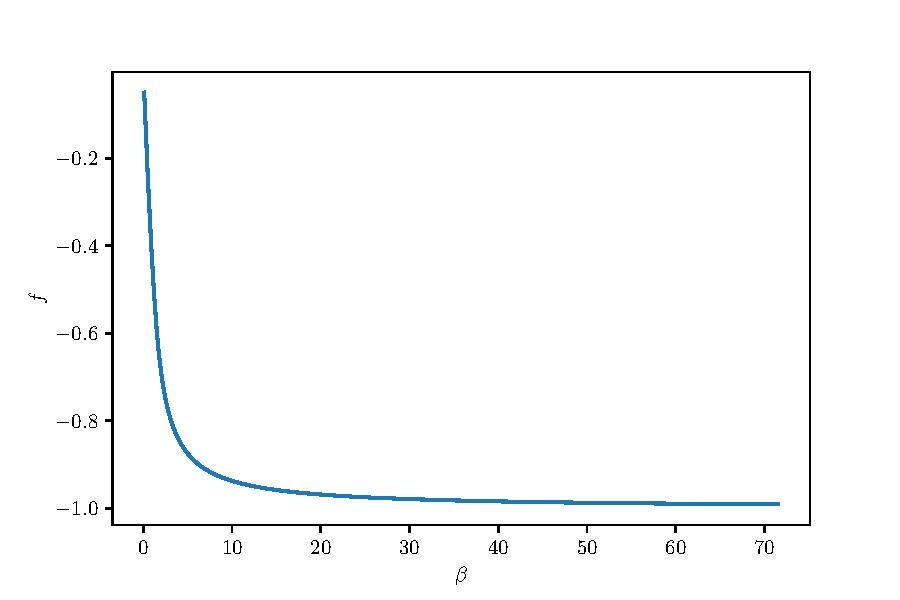
\includegraphics[height=0.65\textheight]{assets/Elibre}
	\caption{\'Energie libre par n\oe{}ud en fonction de $T$}
	\label{fig:elibre}
\end{figure}
\end{columns}
\end{frame}

%
\subsection{En dimension supérieure à deux}
%

\begin{frame}
    \begin{itemize}
        \item La preuve de l'existence d'une transition de phase en dimension supérieure à $2$ demeure un problème difficile (Lars \bsc{Onsager})
        \item Pas de solution analytique en dimension $3$
    \end{itemize}
    Mais une approche numérique permet de comprendre le comportement du modèle d'\bsc{Ising} en dimension supérieure à $2$.
\end{frame}

%%%
\section{Approche algorithmique}
\subsection{Généralités}
%%%

\begin{frame}
Pour réaliser un échantillonnage préférentiel, la chaîne de Markov doit vérifier
\begin{enumerate}[(i)]
	\item Ergodicité : à partir d'une configuration de mesure de Gibbs non nulle, toutes les autres configurations sont atteignables
	\item \'Equilibre détaillé : $P_AW(A \to B) = P_BW(B \to A)$ où $P_A$ est la probabilité d'être dans la configuration $A$ et $W(A \to B)$ est la probabilité de passer de la configuration $A$ à la configuration $B$.
\end{enumerate}
On décompose $W(A \to B) = T(A \to B) \cdot A(A \to B)$ où $T$ est la probabilité que la transition soit proposée et $A$ celle qu'elle soit acceptée.

L'objectif est d'avoir $P_A = \mu(A)$. D'après (ii), cela nous donne 
\begin{align*}
\frac{T(B \to A)\cdot A(B \to A)}{T(A\to B)\cdot A(A \to B)} &= \frac{P_A}{P_B} = e^{-\beta{H(A) - H(B)}}
\end{align*}
\end{frame}

%
\subsection{L'algorithme Metropolis-Hastings}
%

\begin{frame}
	On considère les uniquement transitions par inversion d'un spin avec \[T(A \to B) = T(B \to A) = \frac{1}{\left|V_G\right|}\]
	Algorithme \bsc{Metropolis-Hastings} :
	\[
	A(A \to B) = \min\left(1, \frac{P_B}{P_A}\right) = \min\left(1, e^{-\beta(H(B) - H(A))}\right)
	\]
	Et
	\[
	H(\sigma_i) - H(\sigma_{\overline{\imath}}) = 2J\sigma(i) \sum_\text{$j$ voisins de $i$} \sigma(j)
	\]
\end{frame}

%
\subsection{Résultats}
%

\begin{frame}
\begin{figure}
	\centering
	\begin{subfigure}{0.5\textwidth}
		\centering
		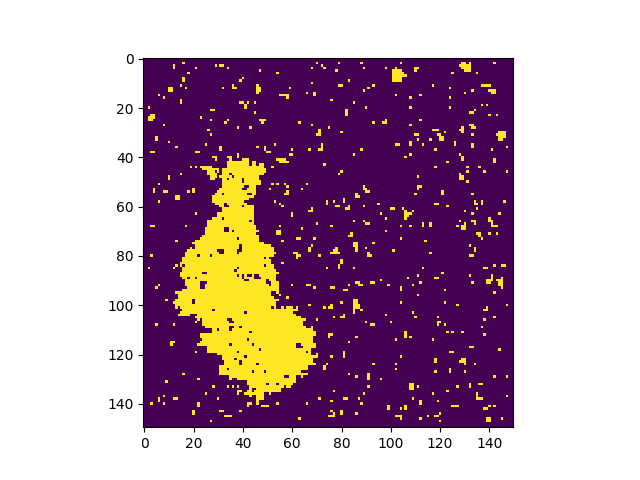
\includegraphics[height=0.55\textheight]{assets/T2}
		\caption{$T = 2$}
		\label{fig:t2}
	\end{subfigure}%
	\begin{subfigure}{0.5\textwidth}
	\centering
	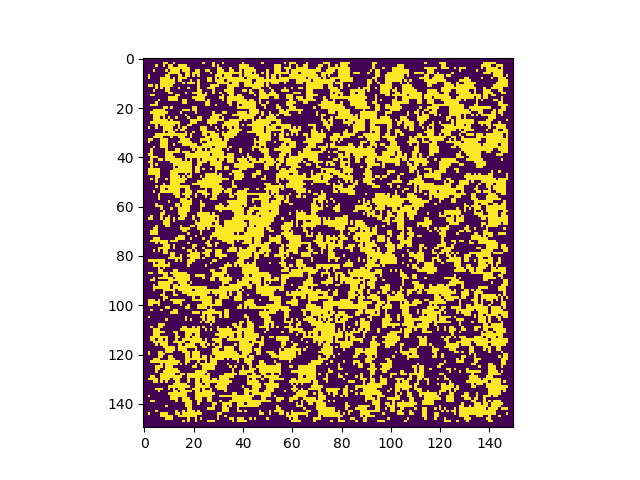
\includegraphics[height=0.55\textheight]{assets/T3}
	\caption{$T = 3$}
	\label{fig:t3}
\end{subfigure}%
\caption{Modélisation numérique : système après \nombre{1000} balayages}
\end{figure}

\end{frame}
\begin{comment}
Mesure de probabilité  du modèle d'ising

\left\langle X \right\rangle_\beta^f = 1 / Z_\beta^f \sum_\sigma X(\sigma) \exp(_\beta H((\sigma))

\end{comment}
\begin{comment}
    Pour condition de bords :
    \[\forall \sigma \in \left\{-1, +1\right\} \qquad H^+(\sigma) = - \sum_\text{$i$, $j$ voisins} \sigma(i)\sigma(j) - \sum_{i \in \text{bord}} \sigma(i)\]
    magnétisation spontanée : inf sur n des < sigma 0 >+ (<- avec cond° bord plus)
    -> brise la symétrie inf_n < sigma 0>^+ > 0 (la magnétisation spontanée : valeur "moyenne" (mesure de probabilité) de sigma0, 
    avec condition bord libre mag = 0, avec cond +, favorise +)
\end{comment}


    %\nocite{*}
    %\printbibliography
\end{document}
